\chapter{Descripción del Trabajo}
\label{cap:descripcionTrabajo}

El desarrollo de este sistema heterogéneo se plantea de forma modular e incremental para
aislar posibles fallos. A continuación, se detalla la metodología de diseño, dividida en
cinco fases técnicas, partiendo desde la configuración inicial hasta la inferencia del
modelo neuronal y su evaluación.

\section{\nohyphens{Configuración del entorno y preparación\\(Fase~1)}}
Antes de comenzar con la lógica del proyecto, es imperativo establecer un entorno de
trabajo sólido. Las herramientas seleccionadas son AMD Vivado (para el diseño hardware) y
AMD Vitis (para el desarrollo del software en \texttt{C}/\texttt{C++}).
Esta primera toma de contacto tendrá como fin crear una aplicación funcional básica para
comprobar el correcto funcionamiento del entorno de trabajo, comunicación con la placa de
desarrollo y comprobación de ejecución.
La lógica programable se configurará para encender unos \ac{LED} con unos pulsadores. Con
esto comprobaremos de forma fácil que la parte \ac{FPGA} de la placa se llega a programar y
que es independiente de la \ac{CPU}.
En la figura~\ref{fig:zybo-1} se muestran los \ac{LED} encendidos correspondientes a los
pulsadores presionados.

\begin{figure}[h]
  \centering
  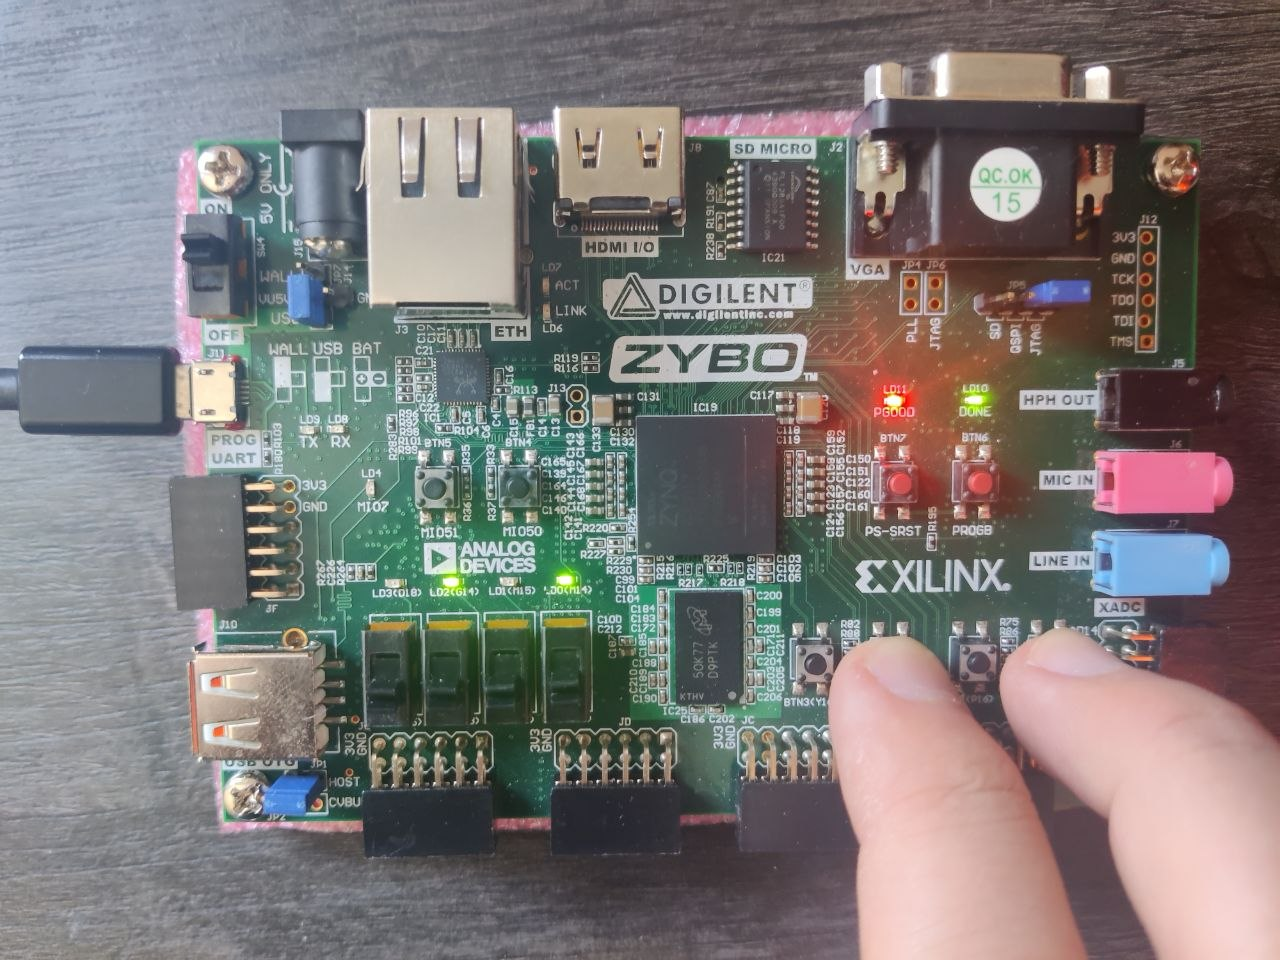
\includegraphics[width=\textwidth]{Imagenes/Bitmap/zybo_phase1.jpg}
  \caption{Imagen de la Digilent Zybo}
  \label{fig:zybo-1}
\end{figure}

El diseño de bloques para esta primera fase puede observarse en la figura~\ref{fig:blockDesign-1}.

\begin{figure}[h!]
  \centering
  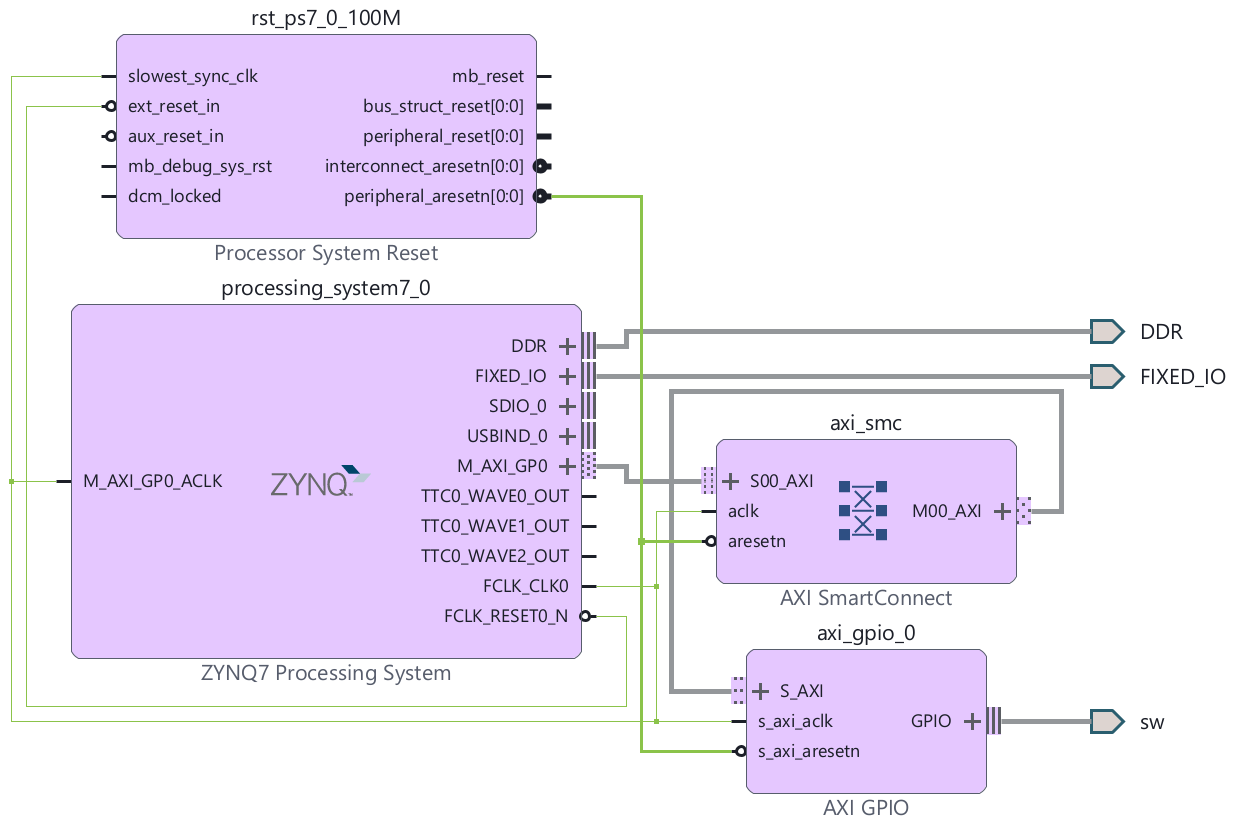
\includegraphics[width=\textwidth]{Imagenes/Bitmap/block_design_phase1.png}
  \caption{Diseño de bloques para encender LED con pulsadores}
  \label{fig:blockDesign-1}
\end{figure}

Después el \ac{PS} tendrá que mostrar unos mensajes por la terminal
serie, leer los interruptores físicos de la placa dos veces, interpretar los números
binarios de los interruptores, sumarlos y mostrar el resultado. Esto hace que comprobemos
que nuestro programa en lenguaje C pueda leer correctamente los \ac{GPIO} de la placa y que
hay comunicación por el puerto serie para la terminal.

Los pasos iniciales son:

\begin{enumerate}
  \item \textbf{Instalación de Board Files y fichero de restricciones:} descargar los archivos de
    definición de la placa Zybo Zynq Z-7010 desde el repositorio oficial de Digilent
    \citep{digilentVivadoBoards} e instalarlos en Vivado.
    Esto preconfigura los relojes, las memorias \ac{DDR} y los pines
    del \ac{SoC} específicos de esta placa.
    Además necesitamos un fichero de restricciones para que Vivado sepa qué pines físicos
    vamos a utilizar y de qué manera.
    Este paso nos sirve para el resto de las implementaciones que haremos.
  \item \textbf{Diseño del Sistema Base:} en Vivado, se crea un Block Design donde se
    instancia el \ac{IP} <<ZYNQ7 Processing System>>. Se ejecuta la automatización de bloques
    (\textit{Block Automation}) para aplicar la configuración de la Zybo. Se añade un
    bloque <<\ac{AXI}
    \ac{GPIO}>> conectado a los \ac{LED} de la placa.
  \item \textbf{Generación y Exportación:} se genera el \textit{Bitstream} (archivo binario que
    configura la \ac{FPGA}) y se exporta la plataforma hardware (.\ac{XSA}).
  \item \textbf{Validación Software:} en Vitis, se crea un proyecto de aplicación
    baremetal (sin sistema operativo). Se escribe un código sencillo en C que imprime
    texto por el puerto serie (\ac{UART}) y hace parpadear los \ac{LED} mediante registros
    \ac{AXI}-Lite, demostrando que el procesador y la \ac{FPGA} están vivos y comunicándose.
\end{enumerate}

En la figura~\ref{fig:terminal-1} se muestra un ejemplo de la salida de la terminal serie
por \ac{UART}.

\begin{figure}[h!]
  \centering
  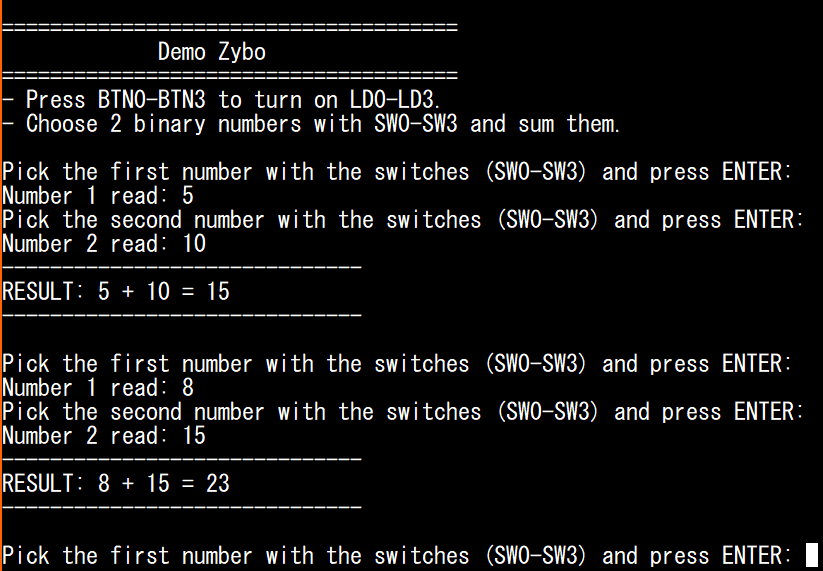
\includegraphics[scale=0.75]{Imagenes/Bitmap/terminal_phase1.png}
  \caption{Salida de terminal correspondiente a la suma de números seleccionados mediante
  los interruptores de la Zybo}
  \label{fig:terminal-1}
\end{figure}

\section{\nohyphens{Comunicación PS-PL (Fase~2)}}
Para el proyecto de aceleración, la \ac{CPU} no puede enviar datos a la \ac{FPGA} dato a dato. Se
necesita un canal directo a la memoria \ac{RAM}.

Para esta fase, hacemos un diseño en el cual las transferencias de datos se realizan por medio
de \ac{DMA}: se lee y se escribe directamente a la memoria \ac{RAM} añadiendo una
conexión \textit{loopback}
directa para validar la ruta completa de comunicación, como se puede ver en la
figura~\ref{fig:blockDesign-2}.

\begin{figure}[h]
  \centering
  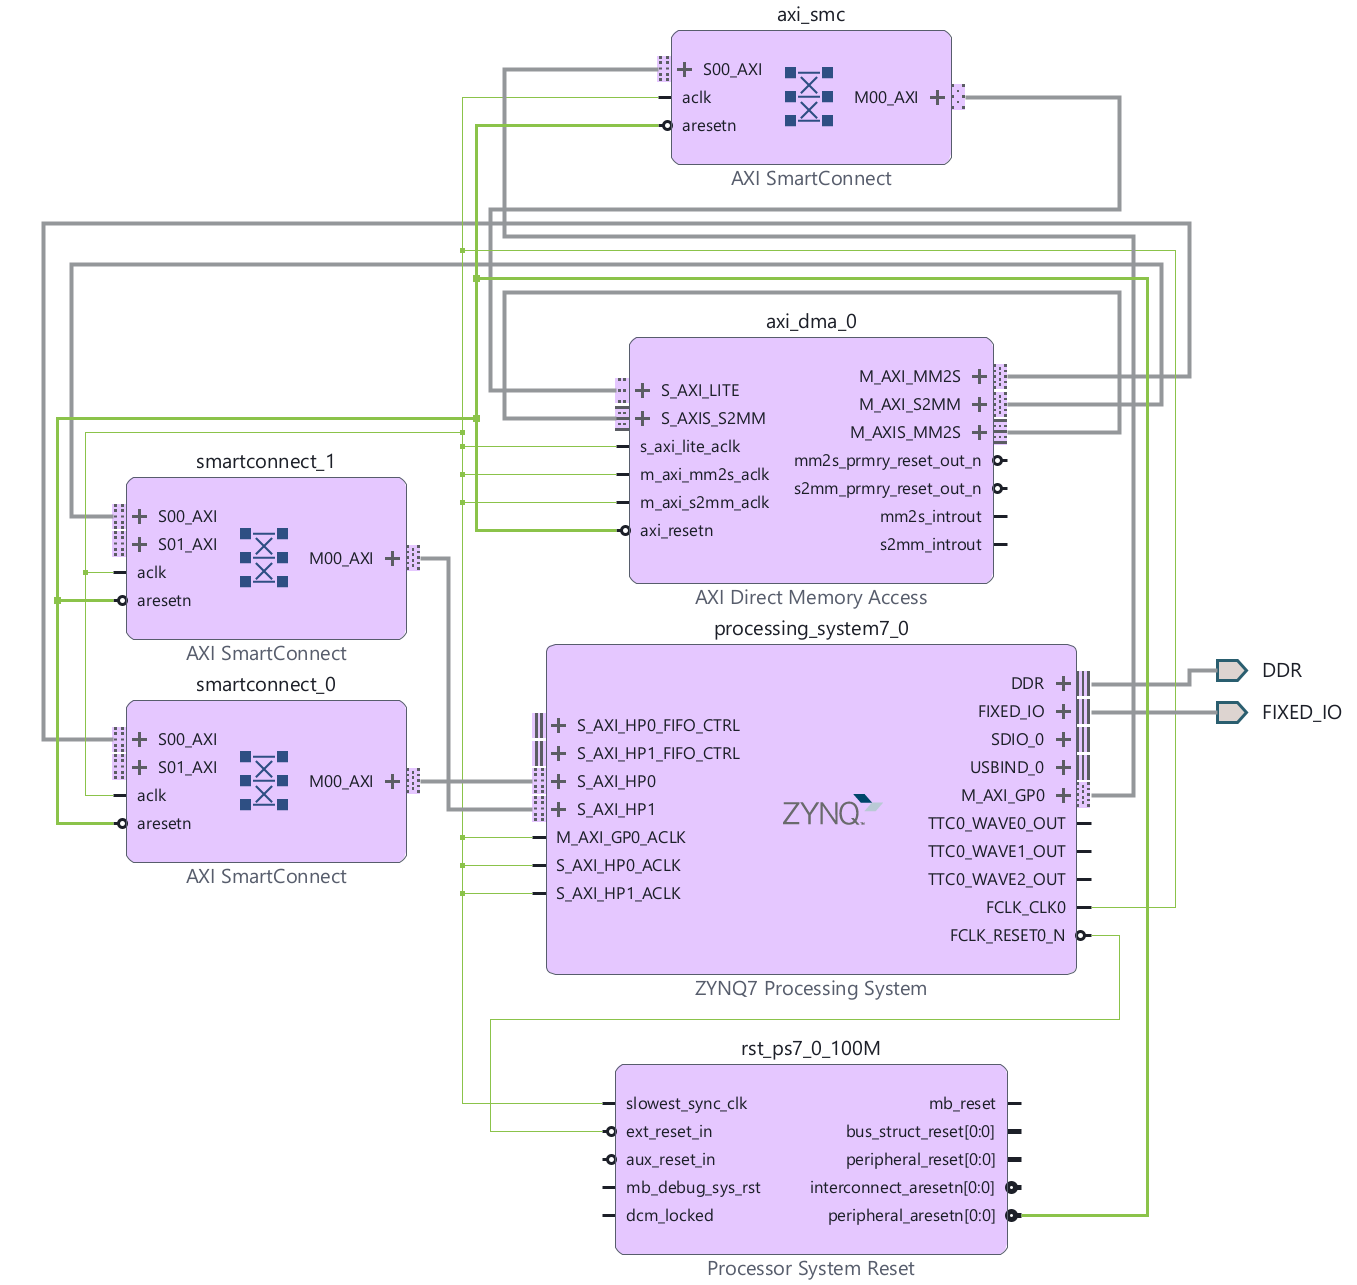
\includegraphics[width=\textwidth]{Imagenes/Bitmap/block_design_phase2.png}
  \caption{Diseño de bloques para validar la comunicación por AXI-DMA}
  \label{fig:blockDesign-2}
\end{figure}

\begin{enumerate}
  \item \textbf{Habilitación de Puertos \ac{HP}:} en Vivado, se modifica la configuración del
    bloque Zynq para activar un puerto esclavo \textit{High Performance} (S\_AXI\_HP0).
  \item \textbf{Integración del \ac{IP} \ac{AXI} \ac{DMA}:} se añade el bloque <<AXI Direct Memory
    Access>>. Se configura deshabilitando la opción \textit{Scatter-Gather} para mantener el diseño
    simple inicialmente \citep{scatterGatherMode}.
  \item \textbf{\textit{Loopback} de Prueba:} para validar el \ac{DMA} antes de
    introducir algoritmos
    complejos, se conecta el puerto de salida del \ac{DMA} (M\_AXIS\_MM2S) directamente a su
    puerto de entrada (S\_AXIS\_S2MM) mediante un bloque FIFO.
  \item \textbf{Software del \ac{DMA}:} en Vitis, se configuran las cachés (definiendo\\
      \texttt{Xil\_DCacheFlushRange} y \texttt{Xil\_DCacheInvalidateRange} para garantizar
      la coherencia de
    los datos entre la caché del \ac{ARM} y la memoria principal) y se lanzan transferencias
    de \textit{arrays} de prueba, validando que el hardware es capaz de mover bloques de datos de
    forma autónoma.
\end{enumerate}

\section{\nohyphens{Desarrollo del acelerador base en HLS:\\multiplicación de matrices (Fase~3)}}
En esta fase del proyecto se ha llevado a cabo el diseño, integración y evaluación de un
acelerador hardware dedicado a la multiplicación de matrices, utilizando metodologías de
codiseño \ac{HW}/\ac{SW}. El objetivo principal ha sido utilizar la \ac{FPGA} con una
tarea altamente
paralelizable y cuantificar la mejora de rendimiento obtenida comparando los resultados
de acelerar el cálculo con la \ac{FPGA} contra realizar el cálculo de forma secuencial en \ac{SW}.

\subsection{Diseño del acelerador mediante HLS}
El desarrollo del núcleo \ac{IP} se ha realizado utilizando la herramienta Vitis \ac{HLS},
permitiendo describir el comportamiento del hardware a partir de un algoritmo en \texttt{C++}.
Para maximizar el rendimiento del sistema generado, se han aplicado directivas de
optimización (Pragmas):

\begin{itemize}
  \item \textbf{Pipeline (\#pragma \ac{HLS} PIPELINE):} implementado en los bucles internos
    para permitir el solapamiento de instrucciones, reduciendo el intervalo de iniciación
    a un ciclo de reloj y maximizando el rendimiento de la ruta de datos.
  \item \textbf{Unroll (\#pragma \ac{HLS} UNROLL):} aplicado para desenrollar total o
    parcialmente las operaciones de multiplicación y acumulación, forzando a la
    herramienta de síntesis a instanciar múltiples bloques \ac{DSP} operando en paralelo.
\end{itemize}

Las interfaces del \ac{IP} core se han configurado bajo el estándar \ac{AMBA} AXI4: puertos
AXI4-Stream para el flujo de datos de alta velocidad e interfaces AXI4-Lite para la
configuración y control desde el procesador principal.

\subsection{Integración a Nivel de Sistema y Arquitectura de Memoria}
El bloque generado se ha integrado en el Block Design de Vivado como se puede observar en la
figura \ref{fig:blockDesign-3}, formando una ruta de
procesamiento completa. Para el movimiento de datos entre la memoria principal y el
acelerador hardware se ha instanciado un controlador \ac{DMA} en modo simple.

\begin{figure}[h]
  \centering
  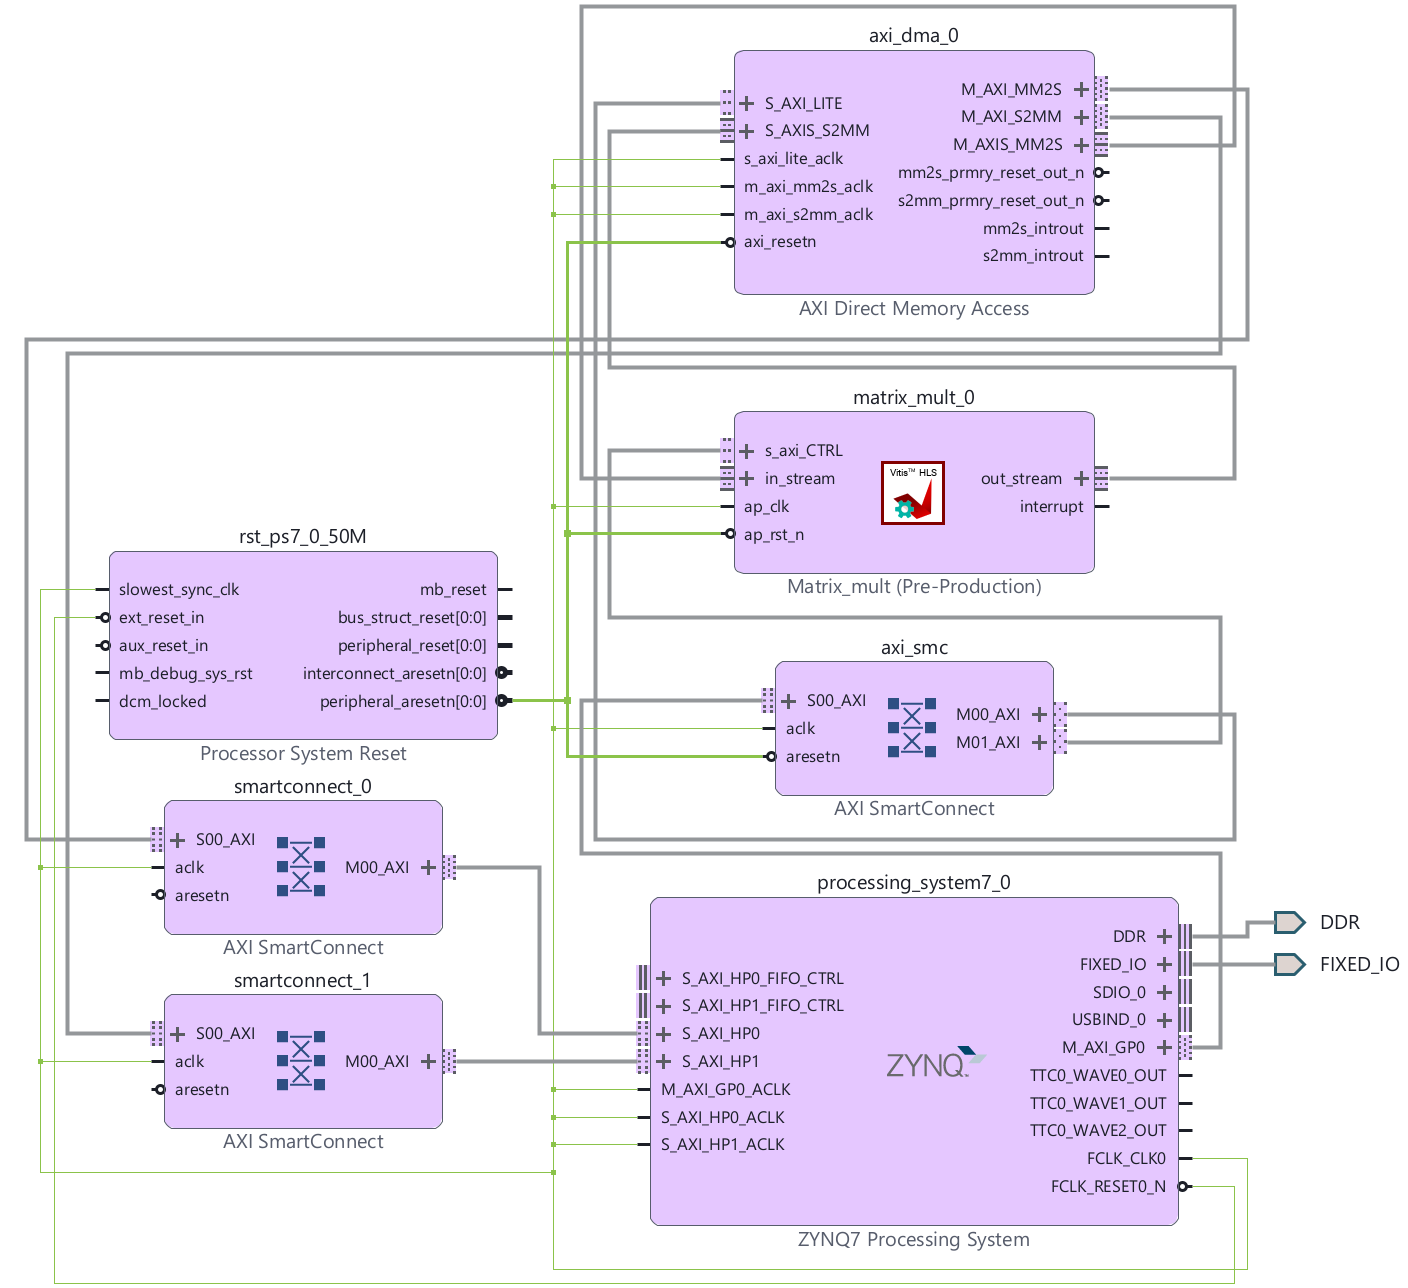
\includegraphics[width=\textwidth]{Imagenes/Bitmap/block_design_phase3.png}
  \caption{Diseño de bloques para la aceleración de multiplicación de matrices}
  \label{fig:blockDesign-3}
\end{figure}

Para evitar cuellos de botella y bloqueos en el bus del sistema, se ha diseñado una
arquitectura de memoria con separación estricta de dominios:

\begin{itemize}
  \item El canal de lectura (\ac{MM2S}) del \ac{DMA} se ha dirigido de forma exclusiva a través del
    puerto de alto rendimiento S\_AXI\_HP0 de la Zynq.
  \item El canal de escritura (\ac{S2MM}) del \ac{DMA} se ha canalizado independientemente a través
    del puerto S\_AXI\_HP1.
\end{itemize}

Esta topología garantiza canales de comunicación dedicados e independientes para la
transferencia bidireccional continua de matrices.

\subsection{Implementación software y coherencia de caché}
El control del sistema se ha desarrollado mediante una aplicación \textit{bare-metal} en lenguaje
\texttt{C}/\texttt{C++} utilizando Vitis IDE. El código ejecuta la inicialización de los
controladores de
hardware y gestiona las secuencias de disparo del \ac{DMA} y del núcleo \ac{HLS}.

Un factor crítico abordado en la capa de software ha sido la coherencia de caché. Dado
que el controlador \ac{DMA} accede directamente a la memoria física y no tiene visibilidad
sobre las cachés L1/L2 del procesador \ac{ARM}, ha sido imperativo ejecutar rutinas de
limpieza (\texttt{Xil\_DCacheFlushRange}) antes de las transmisiones e invalidaciones
(\texttt{Xil\_DCacheInvalidateRange}) previas a las lecturas, asegurando así la integridad de los
operandos y resultados \citep{zynq7000Manual}.

\subsection{Evaluación de rendimiento (Benchmarking)}
Para cuantificar la ganancia de velocidad (\textit{speedup}) real del sistema, se han leído de
forma directa los registros de hardware del \textit{Global Timer} de 64 bits integrado en el
procesador Cortex-A9. Esta técnica evita la sobrecarga de las librerías de tiempo
estándar de C y proporciona una resolución del orden de nanosegundos (basada en el reloj
de 333.33 MHz del temporizador).

Como se puede comprobar en la tabla \ref{tab:resultadosMatrices}, los resultados de las pruebas
de rendimiento demuestran un comportamiento dual dependiente de la carga de datos:

\begin{itemize}
  \item \textbf{Para matrices de dimensiones reducidas (N = 4):} la ejecución puramente
    en software (\ac{CPU}) presenta una latencia menor. Esto se debe al \textit{overhead} o
    penalización temporal implícita en la configuración de los registros \ac{AXI}-Lite del
    \ac{DMA}, el vaciado de las cachés y la latencia propia del bus de interconexión física.
    Para un volumen de datos tan pequeño, el tiempo de comunicación supera al tiempo de cómputo.
  \item \textbf{Para matrices escaladas (N = 32):} a medida que la complejidad
    computacional del algoritmo crece de forma exponencial, el modelo de ejecución
    secuencial del procesador \ac{ARM} sufre una degradación de rendimiento. Por el contrario,
    el núcleo acelerador en la \ac{FPGA} absorbe esta carga gracias al paralelismo masivo de
    los \ac{DSP} instanciados. En este escenario, el tiempo de procesamiento hardware diluye
    completamente el \textit{overhead} de la comunicación por bus, arrojando un \textit{speedup}
    significativo y validando empíricamente la utilidad de la aceleración por hardware en
    operaciones algebraicas intensivas.
\end{itemize}

\begin{table}[h!]
  \centering
  \begin{tabular}{|l|l|l|}
    \hline
    & \textbf{Aceleración \ac{FPGA} ($\mu$s)} & \textbf{Puro \ac{SW} ($\mu$s)} \\ \hline
    \textbf{N=4}  & 5.3680        & 3.3811      \\ \hline
    \textbf{N=32} & 44.8988        & 1338.6451   \\ \hline
  \end{tabular}
  \caption{Resultados en tiempo de la multiplicación de matrices paralelas}
  \label{tab:resultadosMatrices}
\end{table}

\section{\nohyphens{Diseño e implementación del modelo de IA\\(Fase~4)}}
Aunque el planteamiento inicial contemplaba un modelo \ac{MLP} para el
conjunto de datos \ac{MNIST} (28x28 píxeles en escala de grises), la disponibilidad de herramientas
avanzadas de \ac{HLS} permitió elevar el alcance del proyecto.
El diseño derivó hacia una \ac{CNN} capaz de clasificar imágenes a
color de 32x32x3 píxeles correspondientes al \textit{dataset} \ac{CIFAR}-10.

La figura~\ref{fig:blockDiagram-4} muestra el diagrama de bloques simplificado que sigue esta fase
y resume el camino de los datos durante una inferencia completa.

\begin{figure}[h]
  \centering
  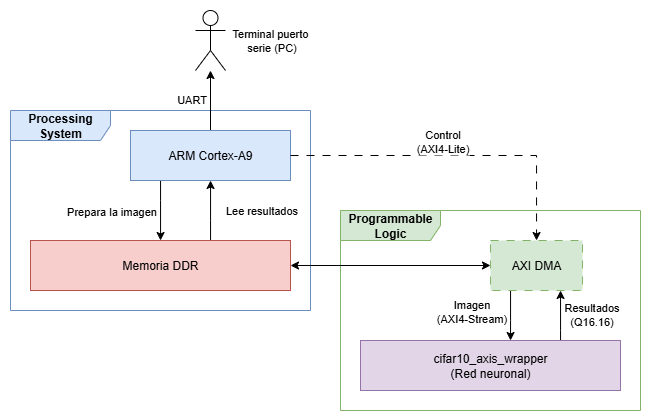
\includegraphics[width=\textwidth]{Imagenes/Bitmap/block_diagram_4.png}
  \caption{Diagrama de bloques conceptual para el funcionamiento de la aceleración de la
  red neuronal}
  \label{fig:blockDiagram-4}
\end{figure}

Dado que la plataforma hardware objetivo es la placa Zybo la cual posee recursos lógicos
muy limitados, el flujo de diseño requirió técnicas de optimización extremas.

\subsection{Entrenamiento y selección del modelo}
El entrenamiento del modelo se realizó en Python con TensorFlow/Keras utilizando un pequeño
código en Python para obtener el modelo entrenado en un formato *.h5. \citep{h5format}.
La red elegida mantiene una estructura sencilla, pero suficiente para extraer
características espaciales de las imágenes \ac{CIFAR}-10:

\begin{itemize}
  \item Dos bloques iniciales formados por convolución 2D y \textit{MaxPooling}, para
    reducir progresivamente el tamaño espacial de la imagen \citep{kerasMaxPooling}.
  \item Una tercera convolución 2D para extraer características de mayor nivel.
  \item Una convolución $1 \times 1$ para mezclar canales sin aumentar demasiado el
    coste de cálculo \citep{lin2014networknetwork}.
  \item Una última convolución $1 \times 1$ con 10 salidas,
    una por cada clase de \ac{CIFAR}-10.
  \item Una capa final \textit{GlobalAveragePooling2D}, que evita utilizar capas densas
    grandes y reduce de forma importante el número de parámetros.
\end{itemize}

Esta decisión fue importante porque las capas densas, aunque son sencillas de programar,
tienden a consumir demasiada memoria y demasiada lógica cuando se llevan directamente a hardware.
En cambio, una arquitectura totalmente convolucional permite conservar la idea de clasificación
de imágenes y, al mismo tiempo, mantener el tamaño del circuito dentro de unos límites razonables.

Durante el desarrollo se probaron varias combinaciones de canales y precisiones.
El primer enfoque que cabía en la placa era demasiado pequeño y ofrecía resultados
de clasificación poco útiles. Después se intentó aumentar el tamaño del modelo y forzar un
mayor uso de \ac{DSP}, pero en la práctica el diseño empezó a fallar en implementación por exceso
de \ac{LUT} o por problemas de empaquetado de \textit{slices}. Finalmente se encontró una
variante intermedia con la siguiente distribución de canales:

\begin{center}
  \textbf{8 / 14 / 32 / 24 / 10}
\end{center}

Estos valores indican el número de canales de salida de cada capa convolucional del modelo.
Cada canal puede entenderse como un mapa de características aprendido por la red.
Por lo tanto, la primera capa extrae 8 mapas de características hasta llegar a la última capa
que contiene 10 canales correspondientes con el número de clases de \ac{CIFAR}-10.

Esta versión consiguió un equilibrio más razonable: el modelo seguía siendo suficientemente
pequeño para implementarse en la Zynq Z-7010, pero mantenía una precisión aceptable
para el alcance del proyecto.

\subsection{Conversión del modelo a HLS}
Una vez obtenido el modelo en formato *.h5, se utilizó hls4ml para traducir la red neuronal
a código \texttt{C++} compatible con Vitis \ac{HLS}. Este paso no consiste solo en
convertir la topología
de Keras, sino también en decidir cómo se representarán los datos dentro del hardware.

El modelo original trabaja en coma flotante, pero esto no es adecuado para una \ac{FPGA} pequeña
como la Zynq Z-7010. Por este motivo se empleó aritmética de punto fijo mediante
tipos \textit{ap\_fixed} \citep{amdPrecisionFixedPoint}.
La entrada y los pesos se redujeron a formatos de pocos bits, mientras
que las acumulaciones internas se dejaron con algo más de margen para evitar
pérdidas graves de precisión.
A nivel de configuración, se utilizó una estrategia orientada a recursos:

\begin{itemize}
  \item \textbf{Strategy = Resource:} prioriza reutilizar operadores frente a generar
    más paralelismo del necesario.
  \item \textbf{ReuseFactor elevado:} permite que las mismas unidades de cálculo se
    reutilicen varias veces, reduciendo el área a cambio de aumentar la latencia.
  \item \textbf{ConvImplementation = LineBuffer:} hace que las convoluciones trabajen con
    \textit{buffers} de línea, una técnica más adecuada para procesar imágenes en flujo.
  \item \textbf{FIFO\_opt activado:} reduce el tamaño de algunas colas internas
    generadas por hls4ml.
\end{itemize}

También se probó a forzar que más multiplicaciones se implementasen usando bloques \ac{DSP}.
Aunque en teoría esto podía liberar \ac{LUT}, en este caso no resultó ser la solución principal.
Al tratarse de multiplicaciones pequeñas, con bastante reutilización y mucha lógica de control
alrededor, mover operaciones a \ac{DSP} no ha reducido el uso total de \ac{LUT}. Por
ello, la versión
final se generó sin forzar explícitamente el uso de \ac{DSP} para todas las multiplicaciones.

\subsection{Adaptación del IP core para AXI DMA}
El código generado por hls4ml no se conectó directamente al sistema, sino que se
encapsuló en un \textit{wrapper} específico.
Este envoltorio adapta la interfaz del modelo neuronal a una comunicación AXI4-Stream,
que es la interfaz natural para conectarlo con el \ac{AXI} \ac{DMA}.

El \ac{IP} core final expone tres tipos de señales \citep{amdAxiDma}:

\begin{itemize}
  \item \textbf{s\_axis:} entrada AXI4-Stream por la que llegan los píxeles de la imagen
    desde memoria \ac{DDR}. Cada palabra tiene 32 bits y representa un valor en formato
    Q16.16\footnote{Q16.16 es un formato de punto fijo de 32 bits. Los 16 bits más
    significativos representan la parte entera y el resto representan la parte fraccionaria.}.
  \item \textbf{m\_axis:} salida AXI4-Stream por la que se devuelven los 10
    \textit{logits}\footnote{Los \textit{logits} representan las puntuaciones brutas sin
    normalizar producidas por la última capa de una red neuronal.} de
    clasificación, también codificados en Q16.16.
  \item \textbf{s\_axi\_CTRL:} interfaz AXI4-Lite de control, generada por Vitis \ac{HLS},
    que permite al procesador arrancar el \ac{IP} mediante \textit{ap\_start} y comprobar
    señales como \textit{ap\_done}, \textit{ap\_idle} y \textit{ap\_ready}.
\end{itemize}

El \textit{wrapper} realiza tres tareas. Primero lee 3072 palabras de entrada,
correspondientes a una imagen de $32 \times 32 \times 3$.
Después alimenta el núcleo generado por hls4ml. Por último, convierte los 10 resultados
del modelo a palabras \ac{AXI} Stream y marca con la señal \textit{TLAST} el último dato de salida.
Esto es necesario para que el canal \ac{S2MM} del \ac{DMA} sepa dónde termina la transferencia.

\subsection{Integración en Vivado}
En Vivado se creó el diseño final con una arquitectura que mantiene la misma idea que
se había validado en las fases anteriores, el procesador \ac{ARM} controla el sistema y
la \ac{FPGA} realiza el cálculo intensivo.

El \textit{Block Design} representado en la figura \ref{fig:blockDesign-4},
integra los siguientes bloques principales:

\begin{itemize}
  \item \textbf{ZYNQ7 Processing System:} contiene el procesador \ac{ARM} Cortex-A9, la
    memoria \ac{DDR}
    y los puertos \ac{AXI} necesarios para controlar el sistema.
  \item \textbf{\ac{AXI} \ac{DMA}:} mueve datos entre la memoria \ac{DDR} y el
    acelerador, evitando que
    la \ac{CPU} tenga que escribir cada dato de forma individual.
  \item \textbf{cifar10\_axis\_wrapper:} \ac{IP} core generado con Vitis \ac{HLS} que ejecuta
    la inferencia del modelo \ac{CIFAR}-10.
\end{itemize}

\begin{figure}[h]
  \centering
  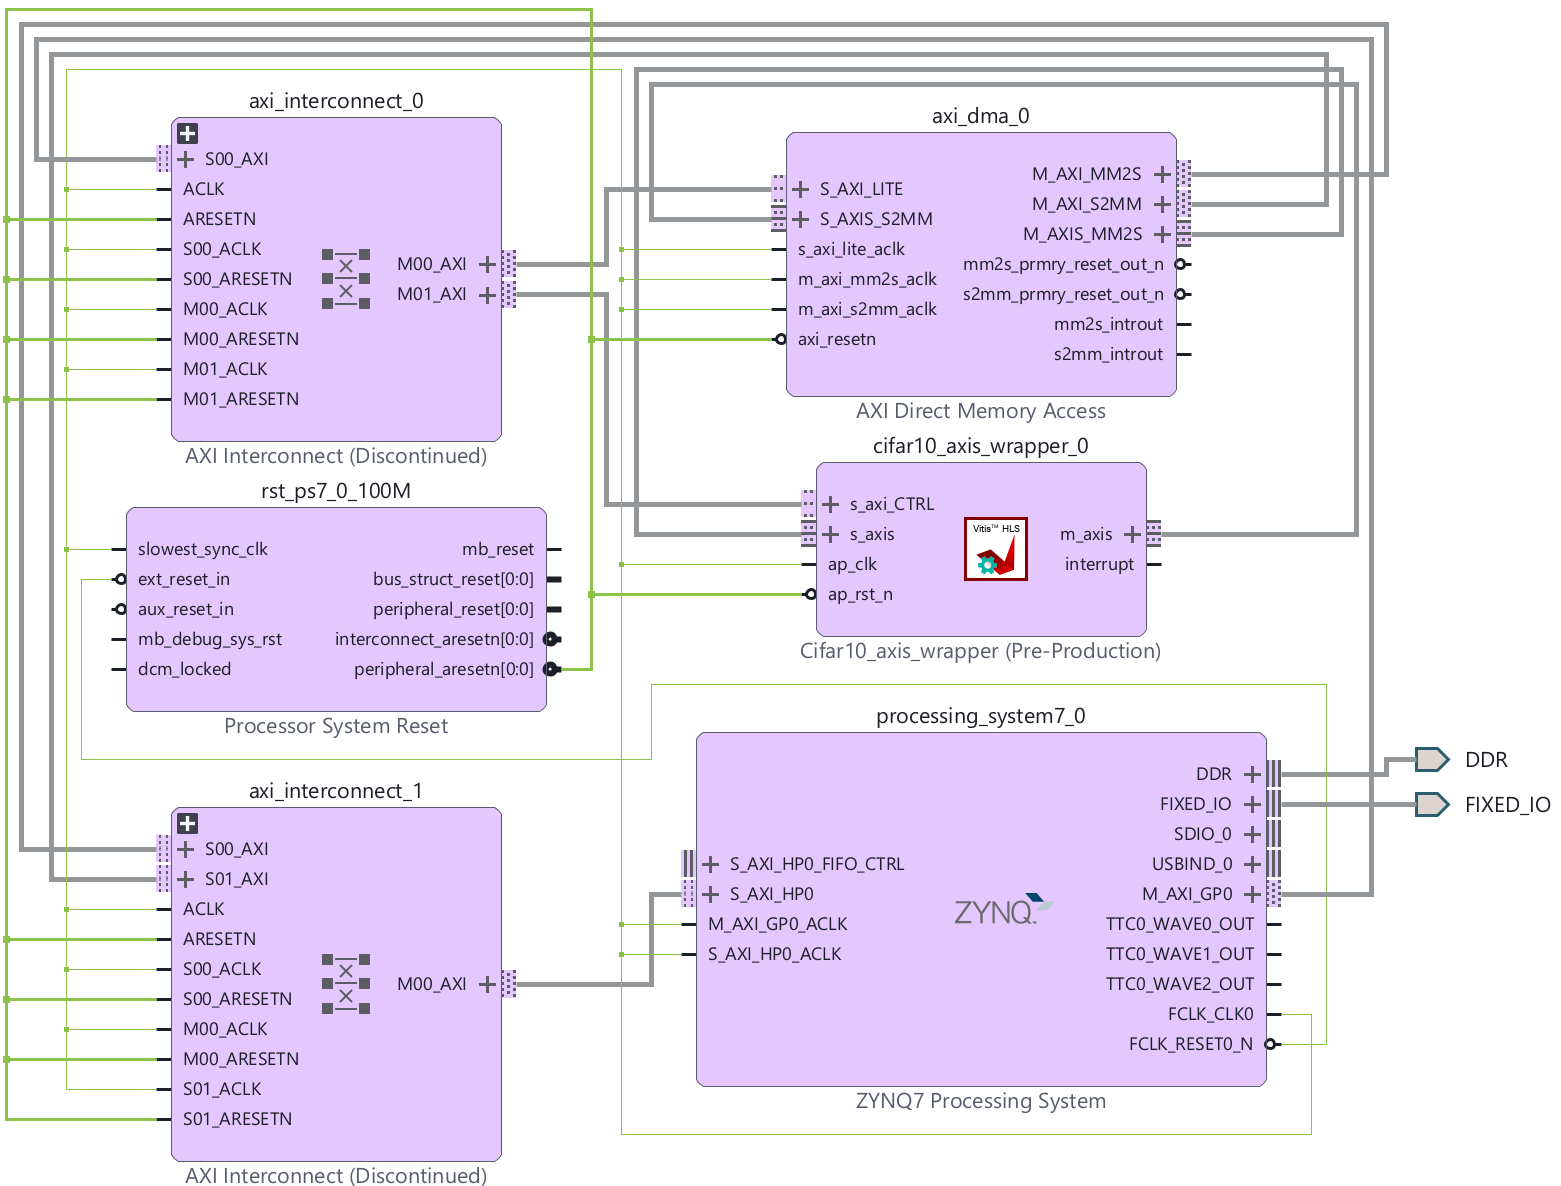
\includegraphics[width=\textwidth]{Imagenes/Bitmap/block_design_phase4_vert.png}
  \caption{Diseño de bloques para la aceleración CNN de CIFAR-10}
  \label{fig:blockDesign-4}
\end{figure}

El recorrido de los datos para este diseño sigue un flujo donde el procesador \ac{ARM} prepara
en memoria \ac{DDR} el \textit{buffer} con la imagen de entrada. Después el canal
\ac{MM2S} del \ac{DMA} lee
la imagen desde \ac{DDR} y la envía al \ac{IP} \textit{cifar10\_axis\_wrapper} mediante
\ac{AXI}4-Stream. Este \ac{IP} recibe la imagen en su puesto \textit{s\_axis}, ejecuta la
inferencia y devuelve los 10 \textit{logits} por el puerto \textit{m\_axis}.
Finalmente, el canal \ac{S2MM} del \ac{DMA} escribe los resultados en la \ac{DDR} desde donde el
\ac{ARM} lee los datos para obtener la clase predicha.

Uno de los puntos más delicados de esta fase fue el ajuste de recursos.
La Zynq Z-7010 dispone de 17600 \ac{LUT}, por lo que pequeños cambios en la arquitectura
del modelo podían hacer que el \textit{bitstream} dejase de generarse. Se probaron varias variantes
que fallaban por exceso de \ac{LUT} o por imposibilidad de empaquetar correctamente las instancias
en los \textit{slices}.

\subsection{Aplicación bare-metal en Vitis}
La aplicación de Vitis se encarga de preparar los datos, arrancar la inferencia y mostrar los
resultados por la terminal serie. Para simplificar las pruebas se incluyeron imágenes \ac{CIFAR}-10
ya convertidas a formato Q16.16 dentro de un fichero de cabecera.
Así, cambiando una macro se puede seleccionar la imagen que se envía a la \ac{FPGA} para probar con
todas las clases de imágenes.

También se puede seleccionar una imagen previamente convertida a un \textit{array} de Q16.16 que se
puede incluir en nuestro código para ejecutar la inferencia sobre esta.
Para ello, se ha incluido un \textit{script} de Python para transformar imagenes en este formato
específico, como se detalla en el capítulo \ref{cap:resultadosEvaluacion} para facilitar
el uso de esta aplicación de inferencia.

La secuencia de ejecución para comenzar la inferencia acelerada por \ac{FPGA} es la siguiente:

\begin{enumerate}
  \item Inicializar el controlador \ac{AXI} \ac{DMA} y comprobar que trabaja en modo simple.
  \item Inicializar el \textit{driver} del \ac{IP} \textit{cifar10\_axis\_wrapper}.
  \item Copiar la imagen seleccionada al \textit{buffer} de entrada y limpiar el
    \textit{buffer} de salida.
  \item Hacer \textit{flush} de la caché para que el \ac{DMA} vea los datos correctos en
    memoria \ac{DDR}.
  \item Iniciar primero la transferencia \ac{S2MM}, para que el \ac{DMA} esté preparado para
    recibir los resultados.
  \item Arrancar el \ac{IP} \ac{HLS} mediante la señal \textit{ap\_start}.
  \item Iniciar la transferencia \ac{MM2S} para enviar la imagen hacia la \ac{FPGA}.
  \item Esperar a que terminen \ac{MM2S}, \ac{S2MM} y el propio \ac{IP}.
  \item Invalidar la caché del \textit{buffer} de salida antes de leer los \textit{logits}.
\end{enumerate}

La gestión de caché es crítica, si el procesador conserva datos antiguos en caché, el \ac{DMA} puede
leer una imagen incorrecta o el software puede imprimir resultados que no corresponden
con la inferencia recién ejecutada.
Por eso se utilizan llamadas explícitas a
\texttt{Xil\_DCacheFlushRange} e \texttt{Xil\_DCacheInvalidateRange}.

\subsection{Interpretación de la salida}
El modelo no devuelve directamente el nombre de una clase, sino 10 valores numéricos llamados
\textit{logits}. Cada \textit{logit} representa la puntuación asociada a una clase de \ac{CIFAR}-10.
La predicción se obtiene seleccionando el índice con el valor más alto, es decir,
aplicando una operación \textit{argmax}.

Para que la salida por terminal sea más comprensible, la aplicación calcula una confianza
aproximada mediante una versión simplificada de \textit{softmax}
\citep{pmlr-v70-guo17a}. Primero se resta el
mayor \textit{logit} a todos los valores para evitar desbordamientos. Después se aproxima la
exponencial y se normalizan los resultados para que sumen el 100\%. Esta confianza no
forma parte del \ac{IP} hardware, sino que se calcula en el programa de test para facilitar la
lectura de los resultados.

Los valores se imprimen en formato hexadecimal, entero con signo y aproximación decimal.
Por ejemplo, un valor Q16.16 divide la palabra de 32 bits en 16 bits para la parte entera
y 16 bits para la parte fraccionaria. Por tanto, para interpretar un \textit{logit} se toma el
entero con signo y se divide entre 65536.

\subsection{Problemas encontrados durante la integración}
Durante la integración apareció un problema especialmente importante: Vivado y Vitis
podían conservar versiones antiguas del \ac{IP} core aunque se hubiese generado una versión
nueva con el mismo nombre. Esto provocaba que el \textit{bitstream} pareciera correcto, pero la
placa seguía ejecutando una versión anterior del acelerador y los resultados de
inferencia eran incoherentes.

La solución pasa por limpiar los productos generados en Vivado, retirar el \ac{IP}
antiguo del diseño,
volver a añadir el repositorio del \ac{IP} actualizado, generar de nuevo el \textit{bitstream},
exportar el fichero \ac{XSA}.
En Vitis la solución es eliminar la plataforma y aplicación, volverlas a generar de
cero añadiendo el correspondiente fichero \ac{XSA} y lanzar \textit{build}.
Tras esta limpieza, la ejecución sobre la placa empezó a devolver \textit{logits}
coherentes con el modelo entrenado.

Otro problema muy común es el límite de caracteres de Windows para las rutas de ficheros.
Cuando una ruta supera los 256 caracteres, la \textit{build} de Vitis o Vivado falla.
Algunas herramientas de Vivado/Vitis generan ficheros que superan este límite, siendo imposible
de mover estos ficheros a rutas más cortas.
Una alternativa habría sido trasladar el espacio de trabajo a Linux, sin embargo, dado que todo
el entorno estaba estaba configurado sobre Windows y las herramientas funcionaban correctamente,
se optó por utilizar el comando \textit{\textbf{subst}}
para asociar la ruta del proyecto de Vivado/Vitis a una letra de unidad de Windows, haciendo
la ruta lo más corta posible.

\section{Pruebas y benchmarking (Fase 5)}

La última fase del proyecto se planteó como una fase de validación. Después de tener el \ac{IP}
\ac{CIFAR}-10 integrado en Vivado y una aplicación \textit{bare-metal} capaz de
comunicarse con él, era necesario
preparar un entorno de pruebas que permitiese medir tiempos, repetir ejecuciones y comprobar que
los datos enviados a la \ac{FPGA} eran exactamente los esperados. Se puede observar la salida
de la terminal en la figura~\ref{fig:terminal-5}.

\begin{figure}[H]
  \centering
  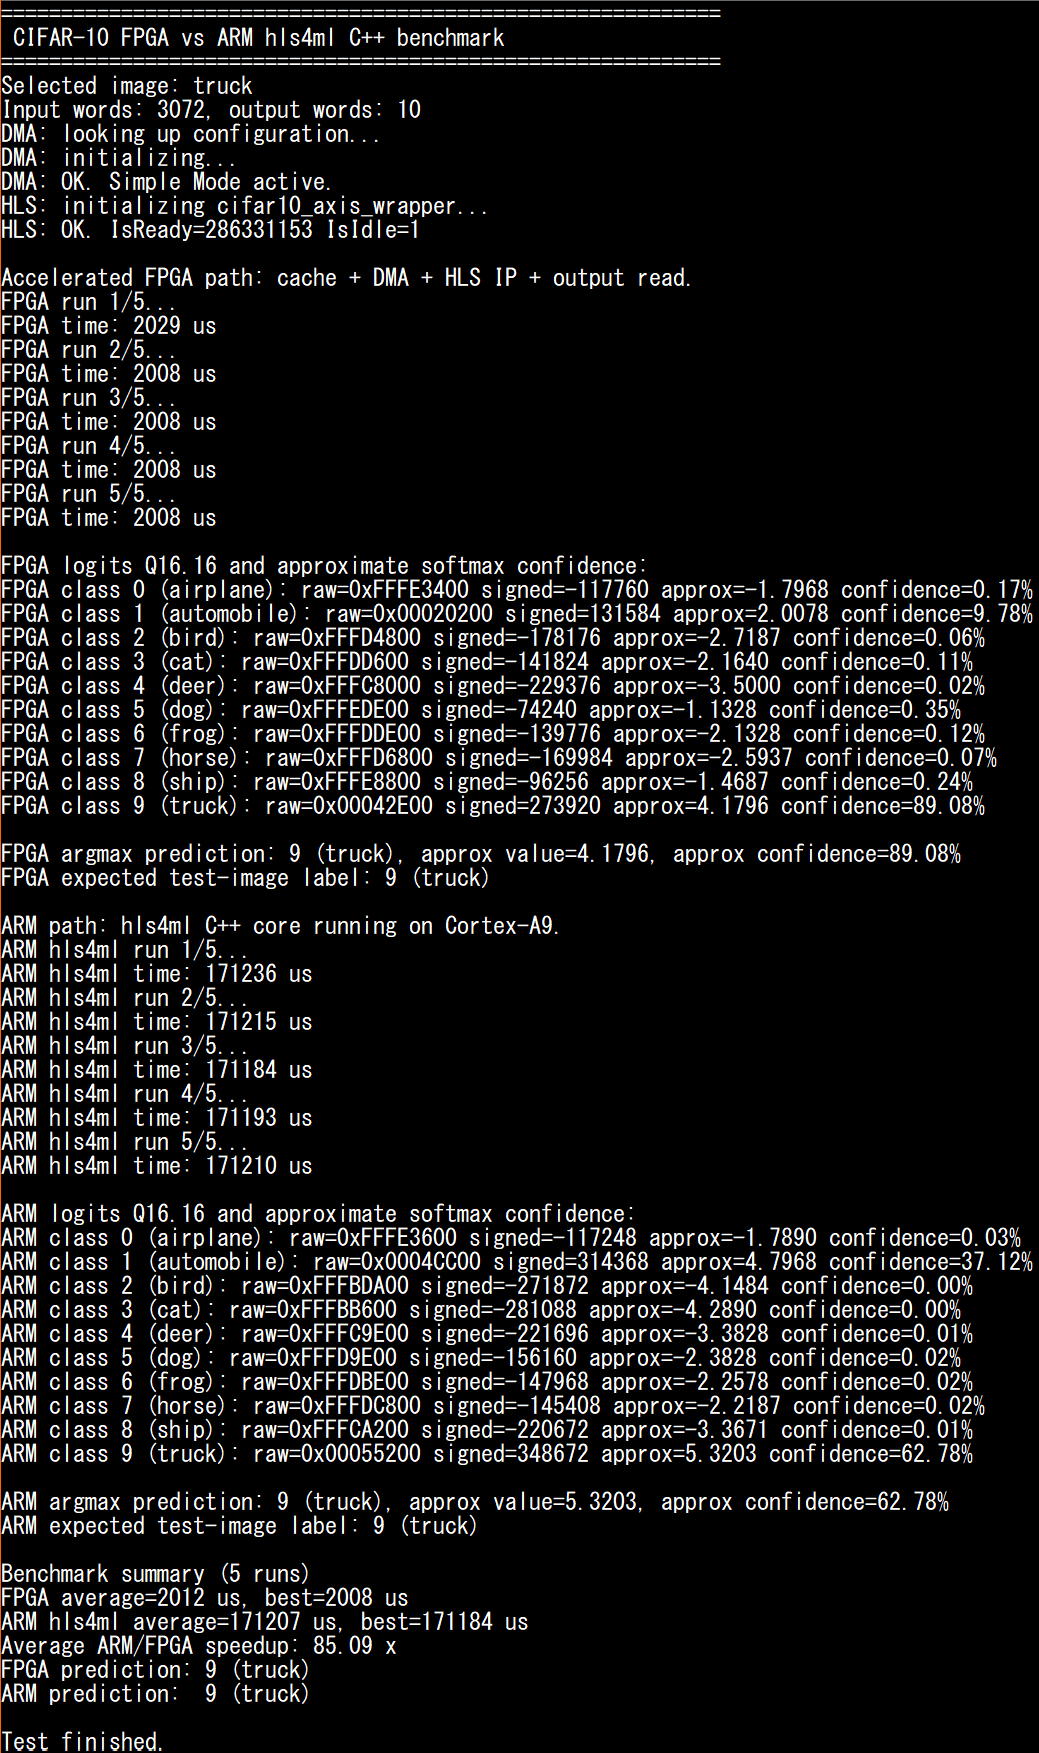
\includegraphics[scale=0.75]{Imagenes/Bitmap/terminal_phase5.png}
  \caption{Salida de terminal con la comparación de inferencia CIFAR-10 ejecutada en FPGA y en ARM}
  \label{fig:terminal-5}
\end{figure}

\subsection{Preparación de pruebas de recursos}
Además de la primera prueba de rendimiento correspondiente a la fase 3, donde se implementó una
multiplicación de matrices acelerada mediante hardware \ac{FPGA} generada por Vitis \ac{HLS}, es de
especial interés medir el uso de área hardware que hace esta herramienta y compararlo con
el que hace el tradicional diseño en \ac{VHDL}.
Ambas fueron configuradas para explotar paralelismo mediante varios multiplicadores simultáneos y
para almacenar datos en memoria interna de la \ac{FPGA}. Esta comparación no buscaba mejorar la
funcionalidad de la multiplicación, sino observar cómo repartía recursos Vivado cuando el mismo
problema se describía desde dos niveles de abstracción distintos.

\subsection{Generación de imágenes de prueba en formato Q16.16}
Para probar la red \ac{CIFAR}-10 sobre la placa no bastaba con tener imágenes en formato
convencional.
El \ac{IP} espera recibir 3072 palabras de 32 bits, una por cada canal \ac{RGB} de una
imagen de 32x32
píxeles. Por eso se prepararon \textit{scripts} auxiliares que convierten una imagen en un fichero
\texttt{.h} que puede incluirse directamente en la aplicación de Vitis.

\begin{figure}[H]
  \centering
  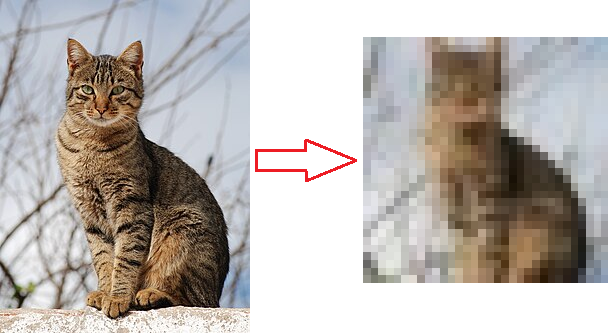
\includegraphics[width=\textwidth]{Imagenes/Bitmap/gato_reducido.png}
  \caption{Imagen reducida con la herramienta image\_file\_to\_h.py}
  \label{fig:gatoReducido}
\end{figure}

El \textit{script} principal es \texttt{image\_file\_to\_h.py}. Este programa recibe una
imagen indicada por
el usuario, la lee mediante TensorFlow, la redimensiona a 32x32 y genera un
\textit{array} en formato
Q16.16. Se puede comprobar un ejemplo de una imagen reducida con el uso de esta herramienta
en la figura \ref{fig:gatoReducido}.

El orden de los datos se mantiene como una secuencia \ac{RGB}:

\begin{center}
  \texttt{pixel0\_R, pixel0\_G, pixel0\_B, pixel1\_R, pixel1\_G, pixel1\_B, ...}
\end{center}

Cada canal se normaliza desde el rango 0--255 hasta el rango [0, 1] y después se escala a Q16.16
mediante la expresión:

\begin{equation}
  \mathrm{valor}_{\mathrm{Q16.16}} =
  \mathrm{round}\left(\frac{\mathrm{canal}}{255} \cdot 65536\right)
\end{equation}

El \textit{script} permite elegir entre varios modos de redimensionado, como \texttt{crop},
\texttt{stretch} o \texttt{pad}. También permite indicar una etiqueta esperada, cambiar el nombre
que se muestra por terminal y guardar una copia de la imagen ya reducida. Esta última imagen fue
útil durante las pruebas, porque permitía comprobar visualmente qué entrada estaba recibiendo
realmente la red neuronal tras el escalado a 32x32.

\subsection{Aplicaciones de inferencia y medición}
Para la inferencia acelerada se encapsuló la comunicación con la \ac{FPGA} en
\texttt{\ac{FPGA}\_cifar10\_accel.c} y \texttt{fpga\_cifar10\_accel.h}. Estos ficheros
inicializan el \ac{AXI}
\ac{DMA}, inicializan el \textit{driver} generado para el \ac{IP}
\texttt{cifar10\_axis\_wrapper}, mantienen la
coherencia de caché y lanzan la transferencia de entrada y salida. La aplicación envía las 3072
palabras Q16.16 por el canal \ac{MM2S} del \ac{DMA} y recibe 10 palabras de salida, una
por clase, por el
canal \ac{S2MM}.

La medida temporal se hizo con el \textit{Global Timer} de la Zynq Z-7010. Este temporizador permite
medir tanto la ruta acelerada como la ruta software con el mismo criterio. En la
ejecución \ac{FPGA} se
mide el tiempo total de una inferencia desde el punto de vista de la aplicación: limpieza de salida,
coherencia de caché, \ac{DMA}, ejecución del \ac{IP} y lectura final del \textit{buffer}.
En la ejecución sobre el \ac{ARM}
se mide el tiempo de ejecución del \textit{core} \texttt{C++} generado por hls4ml sobre
el Cortex-A9.

Para lograr este objetivo, se ha creado un nuevo espacio para el proyecto de Vitis,
\texttt{5\_cifar10\_benchmark}, utilizando el fichero \ac{XSA} y la implementación sobre
\ac{FPGA} de la fase
4. Esta separación deja la aplicación de la fase 4 centrada únicamente en la inferencia acelerada y
reserva la fase 5 para la comparativa entre \ac{FPGA} y \ac{ARM}.

\subsection{Criterios de interpretación}
Las pruebas se interpretan siempre a partir de los \textit{logits} devueltos por el
modelo. La clase final
se obtiene aplicando \textit{argmax}, es decir, seleccionando el índice con mayor puntuación. El
porcentaje de confianza que aparece por terminal se calcula después mediante una
\textit{softmax} aproximada
en la aplicación, por lo que sirve como ayuda de lectura, no como salida directa del
\ac{IP} hardware.

En el capítulo \ref{cap:resultadosEvaluacion} se separan dos tipos de resultados: por un lado, la
validación funcional de la inferencia en la \ac{FPGA}; por otro, el \textit{benchmark}
temporal frente a la
ejecución del \textit{core} hls4ml en el \ac{ARM}. Esta separación evita mezclar el
proceso de preparación del
entorno con la discusión de los resultados finales.
